\section{Break-even controls: a search, a prompt and small policies}
\label{supp:baselines}
Three controls bound every post-training result in this paper, and all three are
cheap to run, and they are reported here in full. All use Benchmark~A v2, identical task rows, and the identical
regret $(\Jobj-\Jobj^\star)/|\Jobj^\star|$ against the strengthened best-known
reference.  They are reported as the mean of per-seed true medians, exactly as the note of Table~I of the main text does.  Every ratio below is therefore formed within one statistic, and
the controls are directly comparable to Sec.~VII-D of the main text, at five seeds.

\emph{(a) A search, with no model at all.}  Gradient-free full-neighbourhood
steepest descent reaches median regret $0.0673$ at feasibility $0.94$ on validation,
$0.2452$
% NOTE: case/policy/inference_search reports 0.0000 for its `steepest_full` arm on the
% same split.  The two are not in conflict and the difference is the stopping rule, not
% the method: inference_search runs to convergence (median 127 forward solves), while
% this arm is capped at --budget 400 with --stall 3 and shares that budget with the
% other arms of the comparison, and on the ood split it needs 312.  Quote 0.0000 when
% the claim is about what search achieves, and 0.0673 when the claim is about what it
% achieves at a matched budget.
at $0.75$ on test and $0.2234$ at $0.62$ out of distribution.  It consumes a median
of $186$ physics evaluations per task (range $30$--$421$). The range exceeds the nominal
$400$-evaluation cap on $9$ of $40$ tasks.  The cap is tested before a round rather
than during one, and a round at $N{=}16$ costs more than the remaining budget.  The comparison is therefore budget-matched to within
one round, not exactly, and is reported that way. Since the oracle that \emph{defines} regret is itself a
search, this is close to the ceiling, and no post-training claim can be a
single-task-quality claim. The defensible claim is amortisation.  Against the same
converged steepest-descent arm of the search case, the measured break-even is
$\sim910$ tasks by
wall clock and $\sim13$ by physics budget.  Both axes are built from the same named
comparator and the same mean statistic.  The budget-capped arm quoted in (a) would
move those to about $3{,}180$ tasks and about $8$ solves, so the break-even is a
property of the comparator, not of the method.  The two differ by two
orders of magnitude because a Benchmark~A solve costs $7$\,ms.  That is precisely the
regime in which the method is unnecessary.

\emph{(b) The same gradient information, as text.} The Introduction's claim that
handing the agent adjoint sensitivities in the prompt wastes information is measured here, and the claim is too strong as written. Injection is not ignored: relative to a plain prompt it improves the warm start
$5.0\times$ on validation ($1.0842\to0.2175$) and $25\times$ out of distribution
($7.4738\to0.2976$).  The model adopts the top-ranked suggested edit in $34$--$86\%$
of rounds on the warm start (per-task follow rate $0.340$--$0.859$) and
$34$--$100\%$ on the frozen base ($0.338$--$1.000$).  It is nonetheless dominated on every split by (a), by $3.2\times$ on validation and
$17\times$ on test.  The feasibility gap is the sharpest part: no single text arm
exceeds $0.50$ on validation, $0.38$ on test or $0.50$ out of distribution, against
$0.94/0.75/0.62$ for the search.  The best text arm also differs by split
($\texttt{steepest\_text}$ at $0.50$ on validation, $\texttt{sens\_exact}$ at $0.50$
out of distribution).  No text arm attains that triple simultaneously. The mechanism is measured rather than assumed.  The search changes exactly $1.00$
decision slots per round, which is all a single-edit linearisation licenses.  The
model changes $0.96$--$3.26$ slots per round on the warm start and $1.00$--$4.80$ on
the frozen base. It applies
the suggested edit \emph{and simultaneously rewrites several others}, and the
injected deltas are first-order in one coordinate at a time with no interaction
terms. Those ranges contain a counterexample to the mechanism as stated.
$\texttt{steepest\_text}$ changes $0.9604$ slots per round on validation and $0.9844$
on test: one edit at a time, exactly what the linearisation licenses.  It still loses
to the search ($0.2175$ against $0.0673$ on validation).  Run to convergence rather
than under the shared budget, the same search reaches median regret $0.0$; the two
search numbers differ only in the stopping rule. Edit discipline is therefore
necessary but not sufficient. Where the model is most disciplined is exactly where the text arms do best.
The information is therefore wasted not because the model cannot read it but
because a text prompt cannot make the \emph{accepted} design the one the linearisation
ranked.  That is a property of the interface, not of the base model.  A better base
model will not fix it. More text is worse, not better: the arm handed the
\emph{entire} simulated neighbourhood loses to the arm handed only the top six edits,
by $28\times$ out of distribution on the frozen base.
% source: ddl/case/llm/E5_prompt_sensitivity/loggers/20260914T204845Z_warmstart and
%         20260914T204845Z_frozenbase, --rounds 30 --G 4 --budget 400 --k 6.
%         follow_rate and hamming_prev per task in results_e5_prompt_sensitivity.json

\emph{The same adjoint as a twelve-solve greedy.}  Ranking the full
neighbourhood by the exact adjoint's first-order prediction and taking its best edit
reaches regret $0.153$ / $0.097$ / $0.076$ at feasibility $0.69$ / $0.63$ / $0.75$ for twelve physics solves. An alternating master/subproblem decomposition reaches
$0.0242$ / $0.0169$ / $0.0385$ for $514$--$1{,}111$ solves.  Both beat every learned
designer in this paper on design quality.  The defensible claim for post-training is
therefore amortisation and measurement, not single-task design.
% source: ddl/case/policy/greedy_and_oracle and ddl/case/policy/inference_search
%         (adjoint-greedy and decomposition arms); details in Supplementary Sec. S-II.

Controls (c) and (d) replace the language model with small policies and are
reported in Supplementary Sec.~S-II.  A 6{,}599-parameter factorised policy reaches
regret $15.73$ / $9.47$ / $7.86$ at five seeds: $169\times$ / $298\times$ /
$349\times$ better than an \emph{untransformed} score-function control that
diverges at this learning rate (Supplementary Sec.~S-II). It is $14.5\times$ worse
than the 4B warm start on validation.  Within a single pinned invocation, a
16{,}260-parameter graph policy beats the factorised policy by $5.92\times$ /
$8.41\times$ / $6.20\times$.  It wins feasibility on validation and test (exact McNemar $p=0.00031$ / $0.00091$; exact paired Wilcoxon on regret $p=0.0035$ /
$8.0\times10^{-5}$ / $0.014$).  The mechanism therefore does not require a language
model; what requires one is Supplementary Sec.~S-III.

Whether the agent can honour a constraint stated in English is measured in
Supplementary Sec.~S-III, and it is the only question on which a language model is
the sole candidate. A factorised policy cannot express ``racks R1 and R2 share a
CDU'' without retraining. An unconstrained search cannot express it at all.
The untrained base model satisfies held-out two-constraint draws significantly
better than any interface that cannot read them ($+0.542$ at $p=0.0003$ on
validation and $+0.375$ at $p=0.0042$ on test, against the factorised policy). Out of distribution the verdict is comparator-dependent ($p=0.064$ against
the policy, significant against the search).  Imitation training costs $25$ points
of compliance and removes the significance on both held-out splits.

The five-checkpoint plate of one run is \cref{fig:traj} of this supplement; the census of Supplementary Sec.~S-VII aggregates it.

\emph{(d) A learned surrogate of the solver.}  A per-task MLP (two 64-unit tanh
layers on the one-hot design vector, trained on the log of the hard-compile
objective).  Inside each cell it is trained on $400$ or $1{,}000$ random one-hot designs
and descended with its own gradient for $200$ normalised steps under the same race
protocol as (a) \cite{shahriari2016bayes,jones1998ego,brunton2020ml}.  At five seeds $\times$ five tasks per $N$: relaxed ratio
$0.204\pm0.144$ (sd, \texttt{ddof}=1) / $0.267\pm0.128$ (surr400) and $0.206\pm0.137$ / $0.229\pm0.105$
(surr1000), against $0.124\pm0.043$ / $0.164\pm0.032$ (pathwise) and
$0.236\pm0.070$ / $0.420\pm0.051$ (score-function).  The deployed hard objective is
$1{,}187\pm1{,}410$ / $3{,}032\pm2{,}364$ (surr1000) against $112\pm268$ /
$366\pm590$ (pathwise); held-out relative error $0.58$ / $0.47$ (median $0.62$ /
$0.44$).  Paired exact signed-rank over the $25$ (seed, task) cells per $N$:
surr1000 against pathwise $p=0.012$ / $0.0088$, surr400 against pathwise
$p=0.037$ / $4.5\times10^{-5}$, surr1000 against score-function $p=0.113$ /
$1.2\times10^{-7}$ (method exact\_dp).  The surrogate is directionally useful and
not shippable: its gradient descends the relaxed objective but its hard decodes are
an order of magnitude worse than the adjoint's.
% source: ddl/case/analysis/surrogate_baseline/loggers/20260916T021844Z_gpuserver/
%         results_surrogate.json -> rows[].{ste_t0.5,surr400,surr1000,reinforce}.
%         {relax,deployed}, rows[].surr1000.surr_rel_err; paired tests recomputed with
%         ddl/tools/summarize_runs.py:wilcoxon_signed_rank (exact_dp).

\section{The endpoint of a post-training run is not a stable summary of its recipe}
\label{supp:bstab}
Every table of post-training results in this paper reports a final value, and this section measures what
that convention costs.  Group all $60$ archived run directories on both benchmarks;
$40$ of them carry two or more checkpoints.  Group them by every argument in their
configuration except the run directory, the seed and the start time.  Comparing
realisations at matched evaluation steps then gives two spreads.  They must not
be conflated.  One is the spread \emph{within} a run across its own checkpoints.  The
other is the spread \emph{between} runs of one configuration.

\emph{Within a run.}  Across the $40$ measured runs the endpoint is the best
checkpoint in $8$, and in $3$ of the $27$ runs that carry a done row.  The worst
endpoint on record is $1{,}188\times$ the best checkpoint of its own run, a
Benchmark-B type-wise realisation that diverged mid-training.  Over the thirteen runs
of the two complete five-seed Benchmark-A score-function configurations (a third
group holds three realisations) the endpoint is best in $2$. Endpoint-over-best reaches $10.05$, and the median within-run worst-over-best
ratio over all measured runs is $7.126$.  \textbf{The final
checkpoint is the best one in $8$ of $40$ measured runs and the worst in $2$}.  One pathwise run on the production solver decodes to $109.18$, $452.97$,
$112.69$ and $185.89$ at checkpoints $0$, $50$, $100$ and $150$.  It is therefore
$4.1\times$ worse than its own warm start at step $50$ and within $3.2\%$ of it at
step $100$.

\emph{Between realisations of one configuration.} Two Benchmark-A score-function configurations have five
complete seeds each. At matched steps the decoded objective differs between seeds by up to
\textbf{$9.871\times$} in the first and \textbf{$12.57\times$} in the second, and the spread at the
endpoint is $9.871\times$ and $1.989\times$. On the production solver the same quantity reaches
$69.3\times$ between two seeds of the pathwise arm and $5.541\times$ between two runs of the
\emph{same seed on two different GPUs}, both complete. \textbf{The spread at step $0$ is exactly $1\times$
in every group}, so the divergence is generated by training rather than by initialisation.

\emph{Three consequences for how such a result may be reported.} First, quoting the endpoint understates:
the complete five-seed configurations end up to $10.05\times$ above their own best checkpoint. Second, quoting the best
checkpoint overstates, and is a nine-way maximum taken on the split being reported. Third, an
\emph{unpaired} comparison of two arms' endpoints has a resolution floor of roughly
$300\times$ at a matched step on Benchmark~B and $9.871\times$ between seeds of one
Benchmark-A configuration. This is why every arm comparison in this paper is a paired
per-task test, except the Sec.~VII-C race of the main text, which pairs per seed ($n=5$, the
finest granularity its artefact stores). It also explains why the graph-policy comparison of
\cref{supp:baselines} survives it: a paired Wilcoxon
conditions on seed and task instead of comparing endpoints.

\emph{What this does not say.} It does not say the instability belongs to one estimator.  At five
complete seeds the score-function arm is as unstable as the pathwise one, so no
arm-specific attribution of the instability is made.  The slot routing remains justified only by the bias
measurement, which is direct and unaffected. Nor does it say the recipe cannot be regularised.  A $20$-step single-seed probe of
it resolves no better than $4{,}544\times$, so no finer claim is made.
% source: ddl/case/analysis/run_stability/loggers/20260915T130706Z_gpuserver/
%         verdict.txt lines 45, 62, 109, 125 (combined census: 60 dirs, 40 measured,
%         best-in-8, worst 1,188x, median 7.126, 9.871x and 12.57x between-seed
%         spreads, ~300x unpaired floor); the two single-benchmark runs
%         20260915T091438Z and 20260915T084208Z are its inputs; results_run_stability.json ->
%         groups[].per_step[].max_over_min and runs[].within. The three trust-region cells are
%         ddl/case/llm/V5_warm_anchor/loggers/20260915T071704Z_gpuserver and
%         ddl/case/llm/V4_kl_anchor_probe/loggers/20260915T055837Z_gpuserver.
%         ddl/docs/RESULTS_index.md rows B17 and L13; ddl/docs/FINDINGS_2026-09-15.md s34-s37.
%         The GPU is not in args.json, so the same-seed two-GPU pair is identified from launch records.

\FloatBarrier

\section{Positioning table and post-training step}
\label{supp:position}
% Full-width float: the table gained two columns relative to the draft's Table I.
\begin{table*}[!t]\centering
\caption{Positioning.  ``Adjoint to weights'' means the simulator's Jacobian
reaches the designer's parameters.  That contrasts with its output value reaching
them as a reward or as prompt text, or its sensitivity field reaching them as a
conditioning input.  ``Relaxation is physical'' means every point of the relaxed
design space is a system the solver can simulate.  ``Pathwise bias'' records what
the work establishes about the bias of a first-order/pathwise gradient estimator;
``measured by decision type'' is a measurement on one production solver, not a
bound or a correction}
\label{tab:position}
\footnotesize
\setlength{\tabcolsep}{5pt}
\begin{tabular}{@{}lccccl@{}}\toprule
 & discrete & LLM & adjoint & relaxation & \\
 & structure & designer & to weights & is physical & pathwise bias\\
\midrule
Score-function post-training \cite{shao2024grpo,scidesignbench2026}
  & \checkmark & \checkmark & -- & n/a & none used (unbiased)\\
STE through tokens \cite{grade2026,diffro2025}
  & \checkmark$^{\dagger}$ & \checkmark & -- & -- & variance reported only\\
Amortized discrete inference \cite{hu2023abs}
  & \checkmark & \checkmark & -- & n/a & n/a (no simulator)\\
Differentiable-sim.\ policy gradients \cite{suh2022diffsim,onoda2026ddcg,scheffler2026cfobg}
  & -- & -- & \checkmark & n/a & analysed, switched, corrected\\
Unbiased mixed gradients \cite{hpo2026}
  & \checkmark & -- & \checkmark & -- & unbiased pathwise/SF mixture\\
Physics-driven designers \cite{jiang2019glonet}
  & -- & -- & \checkmark & n/a & n/a (continuous output)\\
Sensitivity-conditioned TO \cite{topotransformer2026}
  & -- & -- & adjoint as \emph{input} & n/a & n/a (continuous output)\\
LLM design agents \cite{ma2024sga,phythesis2025,jadhav2026mechdesigner}
  & \checkmark & \checkmark & -- & -- & none (no gradient)\\
Adjoint pipe-network TO \cite{blommaert2020adjoint,wack2022energy,wack2023gap}
  & \checkmark & -- & \checkmark & \checkmark & n/a (no learning)\\
Penalised fluid TO (Brinkman) \cite{borrvall2003topology}
  & -- & -- & \checkmark & \checkmark & n/a (no learning)\\
Concurrent water-network adjoint \cite{mu2026gga}
  & -- & -- & \checkmark & n/a & continuous parameters, status frozen\\
Trajectory-scored design agents \cite{zhang2026leap}
  & \checkmark & \checkmark & -- & n/a & none (Bayesian reference)\\
Ground-structure TO \cite{dorn1964automatic,zegard2014grand3d,guest2004minimum}
  & \checkmark & -- & -- & \checkmark & n/a (no learning)\\
Topological derivative \cite{sokolowski1999topological}
  & \checkmark & -- & -- & n/a & structural sensitivity theory\\
Neural combinatorial optimisation \cite{vinyals2015pointer,bello2017neural,kwon2020pomo}
  & \checkmark & -- & -- & n/a & none used\\
Grammar-constrained decoding \cite{hokamp2017lexically,post2018fast,willard2023guided}
  & \checkmark & partial & -- & n/a & n/a\\
RL evaluation methodology \cite{agarwal2021precipice,henderson2018matters}
  & -- & -- & -- & n/a & reporting standard adopted here\\
Density-field TO (SIMP) \cite{bendsoe1989simp}
  & -- & -- & -- & No & n/a (continuous field)\\
\textbf{This work}
  & \checkmark & \checkmark & \checkmark & \checkmark & measured by decision type\\
\bottomrule
\multicolumn{6}{@{}l@{}}{\footnotesize$^{\dagger}$discrete text or codec tokens,
not structural design decisions.}
\end{tabular}
\end{table*}

The positioning table (\cref{tab:position}) and the post-training step the main text summarises are given in full below.

\begin{algorithm}[t]
\caption{One post-training step (pathwise)}
\label{alg:stepS}
\begin{algorithmic}[1]
\STATE sample $B$ tasks; for each, decode $G$ designs under the \ddl{} grammar (no grad)
\STATE simulate each hard design: $\Jobj_g$ (logging / GRPO advantage)
\STATE teacher-forced pass $\to$ restricted logits $\ell$ with grad; same pass with adapters disabled $\to$ $\ell^{\mathrm{base}}$
\STATE conditional Gumbel + straight-through $\to$ $y^{\mathrm{ste}}$; $\soft=\rho(y^{\mathrm{ste}})$
\STATE physics forward at $\soft$ (on the solver GPU), adjoint (implicit-function theorem, main text) $\to$ $d\Jobj/d\soft$
\STATE loss $=\frac{1}{BG}\sum\Jobj/s+\beta\,\mathrm{KL}(\ell\|\ell^{\mathrm{base}})+\lambda_r\mathcal L_{\mathrm{replay}}$; backward; clip; AdamW on LoRA
\end{algorithmic}
\end{algorithm}

\section{Additional figures and the decision-type split table}
\label{supp:extrafigs}
The main text cites these objects by their supplementary numbers; this section holds them so that the main text stays within its page ceiling.
% source: floats of this section render from ddl/case/llm/V2_4b_estimators/loggers/ (nine
%         arms), ddl/case/benchB/E1d_edit_ranking/loggers/20260915T150207Z_edit5seed,
%         ddl/case/benchB/E0f_closure_repair/loggers/20260915T201056Z_gpuserver and
%         ddl/case/analysis/v2A_table/loggers/20260915T175120Z_gpuserver.

\begin{figure}[t]\centering
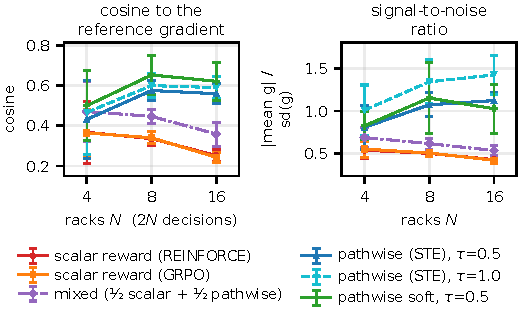
\includegraphics[width=\columnwidth]{figures/fig_e1c_estimators.pdf}
\caption{Gradient-estimator quality versus the number of design decisions on
Benchmark A (mean $\pm$ sd over 5 tasks $\times$ 2 policy points; $S{=}8$
physics evaluations per estimate; reference gradient from 2048 score-function
samples).  Cosine is taken to the reference gradient of the expected objective;
SNR is the norm of the mean estimate over the trace of its covariance.}
\label{fig:e1c}\end{figure}

\begin{figure}[t]\centering
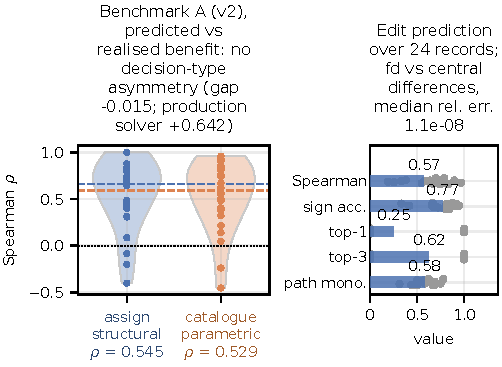
\includegraphics[width=\columnwidth]{figures/fig_e0_edits.pdf}
\caption{Left: per-design Spearman correlation between the first-order
pathwise prediction and the true benefit of every single structural edit (24
checks: six task seeds times four configurations, $N\in\{4,6,8\}$). Right:
aggregate sign accuracy, top-$k$ hit rates and fraction of edits whose objective is
monotone along the relaxation path.}
\label{fig:e0}\end{figure}

\begin{figure}[t]\centering
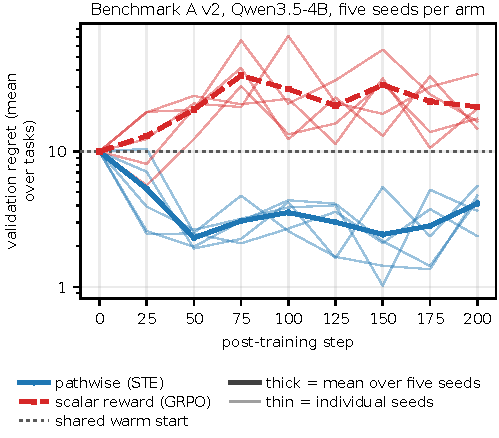
\includegraphics[width=\columnwidth]{figures/fig_e2_v2.pdf}
\caption{Validation regret against post-training step, five
seeds per arm.  Thick lines are the means over five seeds; thin lines are the
individual seeds; the dotted line is the shared warm start.}
\label{fig:e2}\end{figure}

\begin{figure}[t]
\centering
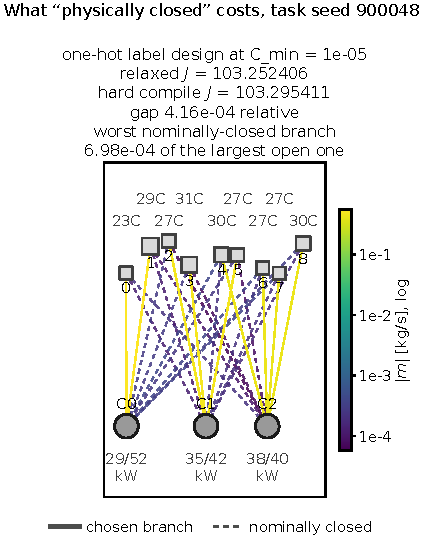
\includegraphics[width=0.86\linewidth]{figures/fig_lc_closure.pdf}
\caption{What ``physically closed'' costs, on one task.  The one-hot label design
evaluated as a \emph{soft} network at $C_{\min}=10^{-5}$ keeps every candidate branch
present with weight at least $C_{\min}$.  The branches a hard network would delete
still carry flow, drawn dashed and coloured on a log scale.  The largest
nominally-closed branch carries $6.98\times10^{-4}$ of the largest open one, and the
relaxed objective differs from the hard compile of the same design by
$4.16\times10^{-4}$ relative.  Both are instances of the floor in
\cref{tab:closure} of this supplementary, whose distance-sweep median at $C_{\min}=10^{-5}$ is
$6\times10^{-4}$.
}
\label{fig:lcclosure}
\end{figure}

\begin{table}[t]\centering\caption{Benchmark B: first-order prediction of a discrete
edit, split by decision type.  The two catalogue relaxations are within noise of each
other ($0.940$ vs $0.939$ rank correlation)}\label{tab:split}
\fontsize{7.2}{8.4}\selectfont
\begin{tabular}{@{}lccc@{}}\toprule
edit type & rank corr. & sign acc. & path monotone\\\midrule
assignment (structural) & $0.31$ & $0.66$ & $0.28$\\
catalogue (parametric) & $\mathbf{0.94}$ & $\mathbf{0.85}$ & $\mathbf{0.78}$\\
\bottomrule\end{tabular}\end{table}

\begin{figure}[t]\centering
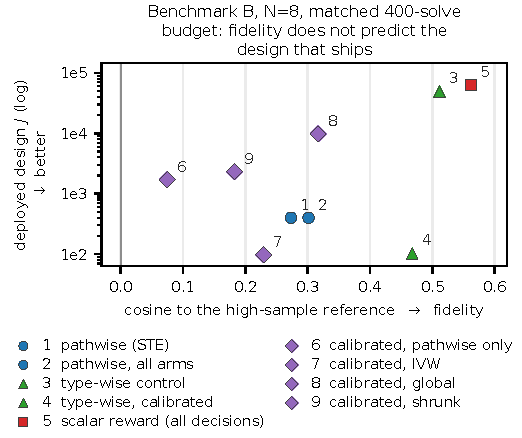
\includegraphics[width=\linewidth]{figures/fig_b_fidelity_vs_deployed}
\caption{The fidelity metric does not predict the design that ships.  Each point is
one estimator arm on Benchmark~B at $N{=}8$ under a matched $400$-evaluation budget:
cosine to a high-sample unbiased reference against the deployed objective of its
argmax-decoded design (log scale, lower better).  The best-aligned arm
($\cos=0.562$) ships $63501$; the pathwise arm ($\cos=0.273$) ships $400$,
$159\times$ better.  Shapes group estimator families; the artefact records nine
arms, eight with distinct deployed objectives.}
\label{fig:bfid}
\end{figure}

\begin{figure}[t]\centering
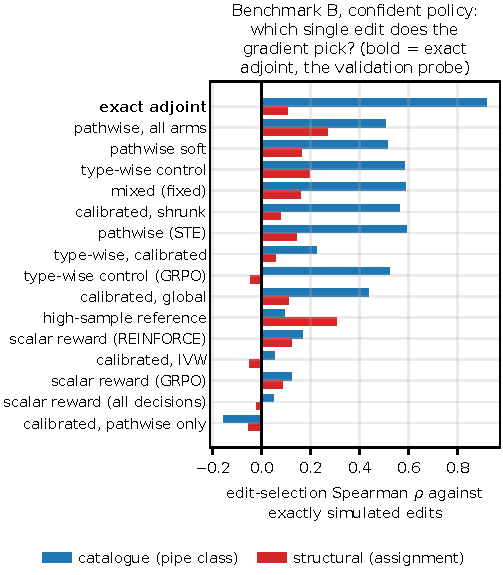
\includegraphics[width=\linewidth]{figures/fig_b_edit_ranking}
\caption{Edit selection at a confident policy point on Benchmark~B, split by
decision type: Spearman correlation between each arm's first-order prediction and the
exactly simulated edit effect, five seeds over ten policy points.  The exact adjoint
reaches $\rho=0.918$ on catalogue edits and $0.104$ on structural ones and picks the
true best edit in $8$ of $10$.  Every stochastic estimator degrades both, and the
scalar-reward arm is uncorrelated with the truth ($+0.0001$).}
\label{fig:bedit}
\end{figure}


\begin{table}[t]\centering\caption{Benchmark B: what the physical-closure floor costs, against a network in
which the unchosen branches are deleted.  Each median is over the five designs
feasible at that $C_{\min}$; the worst leak is the largest nominally-closed branch
flow over the largest open one.  No relaxed solve failed to converge in this sweep.  One hard compile per
$C_{\min}$ is rejected by the topology check: the same dead-end
design at all five floors, because the hard compile does not read $C_{\min}$.  The
pump column is not monotone in $C_{\min}$ ($0.11\%$ at $10^{-5}$ against $0.14\%$
at $10^{-6}$), so the floor is an order-of-magnitude statement.  The $C_{\min}$
column is the dimensionless length and minor-loss weight floor of the production
solver; on Benchmark A the same symbol denotes a conductance floor of
$2\times10^{-5}$\,kg$^2$\,s$^{-2}$\,kPa$^{-1}$}\label{tab:closure}
\fontsize{7.2}{8.4}\selectfont\setlength{\tabcolsep}{3pt}
\begin{tabular}{@{}lcccc@{}}\toprule
$C_{\min}$ & pump power & $\max T_{\mathrm{out}}$ & CDU duty & worst leak\\\midrule
$10^{-2}$ & $3.88\%$ & $1.97$\,K & $19.50\%$ & $80.2\%$\\
$10^{-3}$ & $2.85\%$ & $1.57$\,K & $15.82\%$ & $33.4\%$\\
$10^{-4}$ & $1.00\%$ & $0.71$\,K & $7.11\%$ & $11.4\%$\\
$\mathbf{10^{-5}}$ & $\mathbf{0.11\%}$ & $\mathbf{0.048}$\,\textbf{K} & $\mathbf{1.00\%}$ & $2.15\%$\\
$10^{-6}$ & $0.14\%$ & $0.043$\,K & $0.10\%$ & $0.23\%$\\
\bottomrule\end{tabular}\end{table}

\section{Benchmark-A physicality audit and repair}
\label{supp:audit}
The first physics configuration of Benchmark A admitted non-physical designs that
its own labels made computable.  Enumerating every design of the enumerable sizes
under the legacy configuration gives $13{,}122$ solves with an objective dynamic
range of $1.40\times10^{10}$.  Of these, $414$ designs carry negative rack or pump
flow ($881$ negative rack flows, $403$ negative pump flows).  Under the repaired
configuration (check-valve pump model, $100$\,K temperature cap) the same
enumeration gives a dynamic range of $4.05\times10^{4}$ and $6$ non-physical
designs.  The range reduction is $3.46\times10^{5}$, and the adjoint of the
repaired solver remains exact against central differences.  Sampled designs under
the legacy configuration show a dynamic range of only $1.18\times10^{3}$, which is
why sampling-based checks missed the failure.  The repair is verified against
enumeration wherever enumeration is possible.  On the $12$ of $40$ evaluation rows
small enough to enumerate completely, the best-known reference equals the true
optimum exactly (median, mean, maximum and minimum alike, non-negative fraction
$1.0$).
% source: ddl/case/benchA/E0a_physicality_audit/loggers/20260914T183018Z_gpuserver/
%         results_e0a.json -> enumerated.{legacy|raw, checkvalve|tempered}.
%         {J_dynamic_range, designs_with_neg_flow, neg_rack_flow, neg_pump_flow},
%         sampled["legacy|raw"].J_dynamic_range, verdict.{dynamic_range_reduction,
%         adjoint_still_exact}; enumeration verification from
%         ddl/case/policy/greedy_and_oracle/loggers/20260915T092629Z_gpuserver/
%         results_greedy_oracle.json -> reference_slack.
\section{Benchmark-B post-training: full tables and tests}
\label{supp:e2B}
\subsection{Post-training on the production solver}
\label{sec:e2B}
On Benchmark~B the same recipe trains against the production solver at $48$
training rows against Benchmark A's $64$.  Pathwise and GRPO carry five seeds at
step 200; the type-wise control carries four: its fifth run died at step 178 to a
CUDA device-side assert, is re-running, and nothing here imputes it.  At five seeds
the production solver supplies the paper's sharpest negative: every arm regresses
against its own warm start on regret.  Pathwise is worse on every split in the
pooled per-(seed, task) rows ($p=0.0045$ / $0.00075$ / $0.012$) and inseparable on
the seed-mean primary ($p=0.12$ / $0.18$ / $0.38$).  GRPO is worse on
validation and test on seed-mean ($p=0.034$ / $0.034$), and the type-wise control
diverges ($5.1\times10^{5}$ / $3.2\times10^{5}$ / $879$ against the warm start's
$28$ / $44$ / $69$; seed-mean $p=0.00015$ / $0.0021$ / $0.023$).  Feasibility moves
little and not significantly: pathwise $0.700$ / $0.825$ / $0.650$ against the warm
start's $0.688$ / $0.750$ / $0.625$ (Fisher $p=1$ / $0.49$ / $1$).  A Holm adjustment
over the eighteen seed-mean tests retains five, all of them comparisons against the
diverging type-wise arm.  They are type-wise against the warm start on validation and test,
pathwise against type-wise on validation and test, and GRPO against type-wise on
validation.  Endpoints are not benign either: endpoint-over-best reaches $23$ for
pathwise and $6.4\times10^{5}$ for type-wise (medians $1.47$ / $1.69$ / $37.4$ over
15/15/12 runs).  On the solver where amortisation was supposed to bite,
post-training at 200 steps regresses against imitation training.
% source: ddl/case/analysis/v2B_table/loggers/20260916T033403Z_gpuserver/
%         results_v2B_table.json -> table, paired_wilcoxon (pooled and seed-mean,
%         exact_dp), Fisher counts, endpoint census; type-wise at four seeds with the
%         fifth re-running after a CUDA device-side assert at step 178.
% source: ddl/case/analysis/round10_reanalysis/loggers/20260916T033647Z_gpuserver/
%         results_round10.json -> sec3_holm.benchmark_B.holm_seedmean (5 of 18).
Pooled per-(seed, task) rows give pathwise against the warm start $p=0.0045$ /
$0.00075$ / $0.012$, type-wise against the warm start $p=0.010$ / $7.4\times10^{-5}$
/ $0.0035$, and GRPO against the warm start $p=0.14$ / $0.0019$ / $0.91$.  Pathwise
against type-wise gives $p=0.28$ / $0.00011$ / $0.043$; GRPO against type-wise
$p=0.0031$ / $8.4\times10^{-6}$ / $0.0056$; pathwise against GRPO $p=0.30$ / $0.23$
/ $0.19$.  Feasibility counts: pathwise 56/80, 66/80, 26/40; GRPO 49/80, 45/80,
26/40; type-wise 30/64, 27/64, 16/32; warm start 11/16, 12/16, 5/8.


\begin{figure*}[!t]\centering
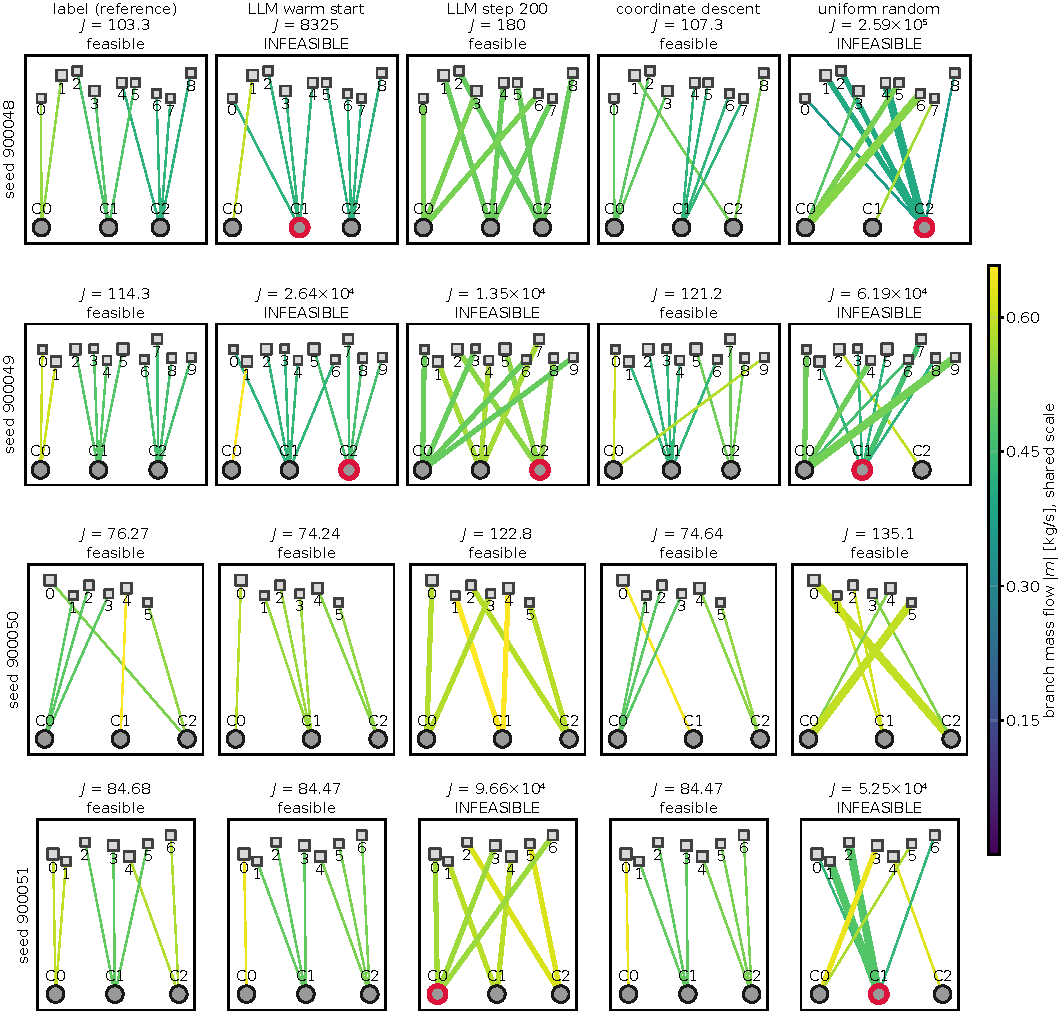
\includegraphics[width=\linewidth]{figures/case_gallery.pdf}
\caption{What each method designs on two Benchmark-B validation tasks (seeds
900048 and 900049); the four-task plate is in the companion repository.  Panels
draw racks (squares, area by heat load) and CDUs (circles); pipe colour and width
are the solved mass flow and the chosen diameter class, and a crimson ring marks
each violated constraint.  The language model was warm-started and post-trained on
Benchmark~B and decoded here unchanged.  Its step-200 design is feasible on one of
these two tasks and never beats two seconds of coordinate descent on either; the
uniform draw is infeasible on both, violating CDU capacity on both.}
\label{fig:galleryS}\end{figure*}

\begin{table*}[t]\centering\caption{Arm-by-criterion matrix on Benchmark~B: gradient-estimate alignment, relaxed descent, shipped design and discrete edit selection at the confident policy point, per estimator arm}
\label{tab:armmatrix}
\footnotesize\setlength{\tabcolsep}{4pt}
\begin{tabular}{l cc cc cc cc}
\toprule
arm & $\cos$ N8 & $\cos$ N16 & relax N8 & relax N16 & deploy N8 & deploy N16 & edit $\rho$ & top-1 \\
\midrule
pathwise (straight-through) & 0.27 & 0.25 & 0.417 & 0.642 & 400 & 397 & 0.477 & 0.80 \\
all-pathwise & 0.30 & 0.29 & 0.417 & 0.642 & 400 & 397 & 0.451 & 0.40 \\
score-function & 0.56 & 0.27 & 0.872 & 0.951 & 63501 & 240837 & 0.000 & 0.20 \\
type-wise & 0.51 & 0.37 & 0.730 & 0.884 & 49334 & 77299 & -- & -- \\
calibrated, global & 0.32 & 0.05 & 0.454 & 0.804 & 9791 & 344 & 0.302 & 0.00 \\
calibrated, shrunk & 0.18 & 0.23 & 0.511 & 0.665 & 2316 & 631 & 0.401 & 0.10 \\
calibrated, IVW & 0.23 & 0.18 & 0.777 & 1.040 & 97 & 103757 & 0.137 & 0.00 \\
soft-forward & -- & -- & -- & -- & -- & -- & 0.448 & 0.10 \\
REINFORCE & -- & -- & -- & -- & -- & -- & 0.156 & 0.10 \\
GRPO & -- & -- & -- & -- & -- & -- & 0.095 & 0.00 \\
\bottomrule
\end{tabular}
\par\medskip
{\footnotesize Cosine is to the reference gradient of the relaxed objective ($n=10$ per cell).  Relaxed descent is final/start relaxed objective, and shipped design the hard-compile objective of the greedy decode, both means over five seeds.  Edit selection is Spearman and top-1 over ten policy points.  Dashes mark criteria an arm was not measured on.  The edit-selection entry of the pathwise row is the deterministic exact-adjoint probe, not the straight-through estimator; the pathwise and all-pathwise rows coincide bitwise on the shipped design.\par}
% source: ddl/case/benchB/E1b_estimator_types/loggers/20260915T150205Z_race5seed_calibbugfix/
%         results_e1b_lc.json -> summary.stats (cos_of_mean, n=10), summary.race (relaxed
%         mean/sd, n=5), race[].greedy[-1][1] (deployed, n=5); edit columns from
%         ddl/case/benchB/E1d_edit_ranking/loggers/20260915T150207Z_edit5seed/
%         results_e1d_edit_ranking.json -> summary[confident|*].
\end{table*}

\section{Solver non-convergence under relaxation: counts, rescues and exceptions}
\label{sec:sxii}
\emph{An engineering observation.}  Relaxing a production solver exposes numerical behaviour that its own design
space never reaches.  The GGA's Newton step fails to converge on a minority of
relaxed designs, entering a non-converging oscillation of the undamped step
near the laminar--turbulent blend.  The failure is not the Jacobian clamp, which floors the conductivity gradient
at $10^{-8}$\,Pa\,s/kg, four orders below the smallest conductivity iterate entry observed.  In the
closure sweep all $90$ relaxed solves converged under the deployed damped Newton
with backtracking and continuation.  The five
failures at $5.6\%$ are hard compiles of a single dead-end design, rejected by the
topology check identically at all five $C_{\min}$ because the hard compile does not
read $C_{\min}$.  The archived rescue counters give the undamped-failure rate where it exists. In the edit-ranking solves of the same run, the archived cumulative counters are
$179$ damped-Newton rescues and $16$ continuation rescues; no per-solve
denominator is archived, so no rate is quoted.
The failures localise in \emph{design} space rather than in $C_{\min}$.  Over
$12{,}800$ relaxed solves drawn at a controlled distance $\varepsilon$ from the
label design, $0$ of $5{,}120$ fail at $\varepsilon<0.1$ and $10$ of $7{,}680$
($0.13\%$) fail at $\varepsilon\ge0.1$.  It never fails at the label design or within
half a decision of it and starts failing once designs are one decision away, which is
part of the regime a post-training run explores.  The three
Benchmark-B arms that completed $200$ steps drew $6{,}400$, $3{,}200$ and $6{,}400$
relaxed solves and recorded \emph{zero} crashes.  A failed sample is not fatal in
any case: the estimator replaces it with the detached mean of the samples that
converged, and returns a zero-gradient step when a whole group fails.  So the honest statement is that non-convergence is rare, and that it is
concentrated beyond one decision from a good design.  The curve says where it lives.
It does not say that a long run must crash: the same paragraph's $0$-of-$5{,}120$
contradicts the stronger claim.
% source: case/analysis/sampling_tail_control/loggers/20260915T051016Z_gpuserver/
%         results_sampling_tail.json -> results[bench=B].relaxed_solver.{n_failed_solves,n_solves};
%         ddl/docs/FINDINGS_2026-09-15.md s30.3. Failure handling follows the trainer's own rule
%         (ste.pathwise_objective substitutes the detached mean of the converged samples).
The solver runs
damped Newton with backtracking and continuation always on and exposes no undamped
mode, so earlier multi-mode ladders were never configurations of a single
measurement.
A genuine three-mode ladder
would require instrumentation flags inside the production solver module, which is
shared with
other work in this repository and was not modified for it.  We report this
at all because it is a cost of the method that a reader adopting it will pay.


\section{Benchmark-A paired-test census behind Table~I}
\label{supp:acensus}
The primary paired test of Table~I of the main text is the exact tie-aware
signed-rank test on one pair per task over the seed-mean regret ($n=16$/$16$/$8$).
Pathwise against GRPO gives $p=0.011$ / $9.2\times10^{-5}$ / $0.0078$; pathwise
against the warm start $p=0.71$ / $0.12$ / $0.0078$; GRPO against the warm start
$p=0.034$ / $0.0092$ / $0.31$.  Type-wise control against the warm start gives
$p=0.94$ / $0.50$ / $0.15$; against pathwise $p=0.27$ / $0.051$ / $0.023$; against
GRPO $p=0.025$ / $4.3\times10^{-4}$ / $0.0078$.  A Holm adjustment over these
eighteen tests retains two: pathwise against GRPO on test and GRPO against
type-wise on test.  The pooled per-(seed, task) convention ($n=80$/$80$/$40$) is
reported beside it as a sensitivity analysis only.  The warm start is one adapter
decoded identically by every seed, and the task axis clusters the cells (ICC up to
$0.95$, effective $n$ as low as $9$ of $40$).
% source: ddl/case/analysis/v2A_table/loggers/20260915T175120Z_gpuserver/
%         results_v2A_table.json -> paired_wilcoxon and paired_wilcoxon_seedmean
%         (wilcoxon_method exact_dp in every cell); Holm from
%         ddl/case/analysis/round10_reanalysis/loggers/20260916T033647Z_gpuserver/
%         results_round10.json -> sec3_holm.benchmark_A.
